\section{Introduction}
\label{sec:intro}


\section{Background}
\label{sec:background}

\subsection{RDMA}

RDMA is a networking technology which allows client machines
to directly access the memory of a remote server. RDMA is an
enabling technology for memory disaggregation as
\textit{memory servers} do not need any computation
resources (save setting up the RDMA memory initially).

One sided RDMA verbs (read, write, atomic) are used to
access remote memory without any memory side computation.
One sided verbs require RDMA reliable connections which
guarantee in-order delivery of operations.


\subsection{Remote Memory Data Structures}

\section{Problems}
\label{sec:problems}

Designing data structures for remote memory is hard. The
primary reason is that there is no centralized serialization
point to guard access to remote memory. Traditional key
value stores (Memcached~\cite{memcached}), and even RDMA
based Key-value stores~\cite{herd,erpc,pilaf} use a mixture
of one-sided and two-sided verbs. Normally writes are two
sided, and the memory-side CPU performs locking close to
memory and ensures that all writes are issued in order.

In remote memory, no such CPU exists. To get serialization
expensive RDMA atomic operations like \textit{compare and
swap}(CAS) must be used. Atomic operations are by no means a
silver bullet. With a CPU close to memory critical sections
are small. Consider inserts into a cuckoo hash table with a
long path. The CPU acquires some number of locks in memory
then performs a series of reads and wites to commit the path
before unlocking. Reads writes and locking only consumes a
memory access ~50ns which keeps the critical section small.
In contrast locking with RDMA atomic operations and
performing multiple lookups is very expensive.

First, acquiring a lock means a round trip. If the table has
a single lock, then a client is guaranteed to be able to
gather all the locks it requires in a single round trip.
However a single lock does not scale as only a single writer
can write at a time. This matter is made worse by the fact
that the critical section of the lock is larger in remote
memory. Breaking the table up into subtables each with it's
own lock has it's own problems. An insertion with a long
path will potentially need to acquire many locks. Each of
which requires a round trip. Therefore using fine grained
locking increases the tables scalability but increases it's
base case insertion time.

\textbf{Read Optimization} Most data center workloads are
read heavy, therefore read operations should be the most
highly optimized~\cite{datacenter-workloads}. Prior
approaches such as RACE require two RDMA round trips per
read. The first is a hash index lookup, the second round
trip reads the actual key-value block. RACE must perform two
round trips because entries in the hash index are limited to
64 bits (CAS width). This is commonly not enough to store
both key and value so RACE can not inline both keys and
values in the index structure. Clover~\cite{clover} enables
single round trips reads. However under contention Clovers
reads require pointer chasing which is known to be expensive
due to each pointer resolution requiring a round
trip~\cite{clio,clover,pointer-chaising}. Ideally we would
be able to ensure that reads complete in a single round
trip.


\section{Design}
\label{sec:design}

\subsection{Locality Hashing}

Cuckoo hashing and Hopscotch hashing are both read optimized
hash tables. Cuckoo hashing ensures that all reads are at
most two memory accesses~\cite{cuckoo}, while hopscotch
hashing ensures that a read is within a bounded range of
it's hash index~\cite{hopscotch}. Both of these properties
have been noticed by the RDMA key-value store, and far
memory communities for their fast
reads~\cite{memc3,cuckoo-improvements,pilaf,farm}.

Our approach aims to combine the bounded reads of cuckoo
hashing, with the locality properties of hopscotch hashing.
To do so we bound the distance between cuckoo hash
locations. Traditional cuckoo hashing calls for two
independent hash functions. We instead make our two hash
functions dependent. The first hash function determines the
location a key will be hashed to. The second hash function
determines the maximum distance the second value can have
from the first. A third hash function determines a random
location between the first location, and the bound imposed by
the second.

A strawman implementation of locality based hashing would
use the first hash function to find a location, and the
second to find a random location within a fixed bound. This
approach quickly leads to failed insertions. Due to the
birthday paradox the probability of a collision is high, and
on large tables the probability that one region of the hash
table will become full, and have not viable path to an open
slot is high. ~\todo{Insert a figure of one of my failed
insertion experiments on a big table}.

Rather than use a static bound we use a dynamic logarithmic
bound. The bound set by the second hash function is
determine by counting the suffix zeros of the resultant hash
and rasing it by an exponential factor. In the common case
the bound is small, but on an exponentially decrease rate
some pairs of values are spaced far apart. This design
enables some pairs to act as ~\textit{waypoints} to other
regions of the table. This method, paired with associative
in the cuckoo hash enables high fill rates while keeping the
region of the table any given key can inhabit
small.

\begin{figure}
    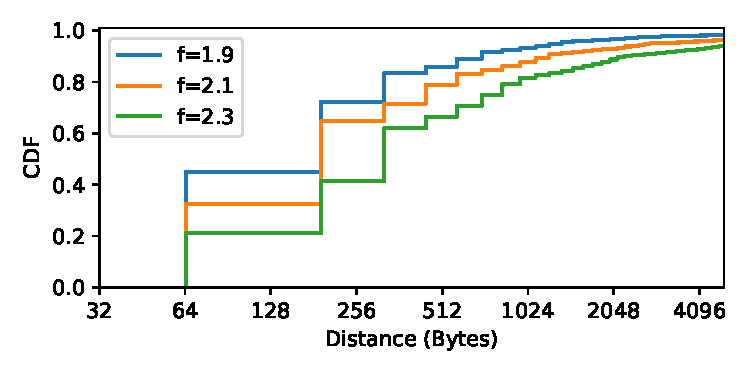
\includegraphics[width=0.99\linewidth]{fig/hash_factor.pdf}
    \vspace{-1em}
    \caption{CDF of distances between cuckoo locations dependent hashing on different exponential factors.}
    \label{fig:hash_factor}
\vskip -1em
\end{figure}

\begin{figure}
\begin{align*}
    L_1 &= h_1(k) \\
    L_2 &= L_1 + h_2(k) \% f^{f + log_2(h_3(k))}
\end{align*}
\caption{Locality based hashing for factor $f$}
\end{figure}

~\todo{Show a figure of the CDF of the hash
functions.}

~\todo{Show a figure of the hashing and how it relates to the table.}

\subsection{Locking}

\subsection{Protocol}


\section{Evaluation}
\label{sec:eval}

\section{Conclusion}
\label{sec:conclusion}
